%% LyX 2.0.2 created this file.  For more info, see http://www.lyx.org/.
%% Do not edit unless you really know what you are doing.
\documentclass[10pt,english]{beamer}
\usepackage{mathptmx}
\usepackage[T1]{fontenc}
\usepackage[latin9]{inputenc}
\usepackage{amsmath}
\usepackage{amssymb}
\usepackage{graphicx}

\makeatletter
%%%%%%%%%%%%%%%%%%%%%%%%%%%%%% Textclass specific LaTeX commands.
 % this default might be overridden by plain title style
 \newcommand\makebeamertitle{\frame{\maketitle}}%
 \AtBeginDocument{
   \let\origtableofcontents=\tableofcontents
   \def\tableofcontents{\@ifnextchar[{\origtableofcontents}{\gobbletableofcontents}}
   \def\gobbletableofcontents#1{\origtableofcontents}
 }
 \def\lyxframeend{} % In case there is a superfluous frame end
 \long\def\lyxframe#1{\@lyxframe#1\@lyxframestop}%
 \def\@lyxframe{\@ifnextchar<{\@@lyxframe}{\@@lyxframe<*>}}%
 \def\@@lyxframe<#1>{\@ifnextchar[{\@@@lyxframe<#1>}{\@@@lyxframe<#1>[]}}
 \def\@@@lyxframe<#1>[{\@ifnextchar<{\@@@@@lyxframe<#1>[}{\@@@@lyxframe<#1>[<*>][}}
 \def\@@@@@lyxframe<#1>[#2]{\@ifnextchar[{\@@@@lyxframe<#1>[#2]}{\@@@@lyxframe<#1>[#2][]}}
 \long\def\@@@@lyxframe<#1>[#2][#3]#4\@lyxframestop#5\lyxframeend{%
   \frame<#1>[#2][#3]{\frametitle{#4}#5}}

%%%%%%%%%%%%%%%%%%%%%%%%%%%%%% User specified LaTeX commands.
\usepackage{multicol}
\usetheme{Madrid} 
\usecolortheme{orchid} 
\setbeamercovered{transparent} 
\setbeamertemplate{navigation symbols}{} 
% DEFINE YOUR LOGO
\newcommand{\mylogo}{
 
\includegraphics[width=1cm,height=1cm,keepaspectratio]{./Desylogo.pdf}~%
 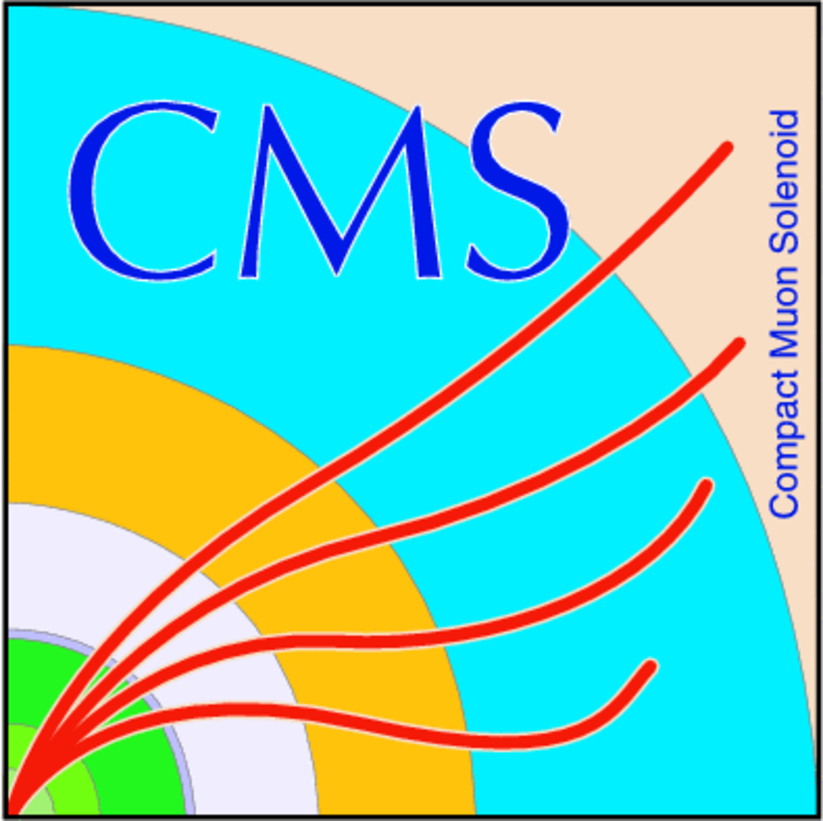
\includegraphics[width=1cm,height=1cm,keepaspectratio]{./CMSlogo.pdf}%
}

\usepackage{url}


\setbeamersize{text margin left=1cm,text margin right=1cm} 
 
% OVERWRITE FRAME DEFINITION
\let\oldlyxframe\lyxframe 
\renewcommand{\lyxframe}[1]{\oldlyxframe{\mylogo\hspace{3mm} #1}}

\makeatother

\usepackage{babel}
\begin{document}

\title{TopSVDFunctions}


\subtitle{Quick Start Guide}


\author{D.~J.~Fischer\inst{1}}


\institute{\inst{1}DESY Hamburg}


\date[9/17/2012]{September 17, 2012}

\makebeamertitle

\lyxframeend{}


\lyxframeend{}\lyxframe{Step 1: Installation}
\begin{itemize}
\item Make sure, C++ standard library and STL are available on your machine.
\item Make sure, ROOT 5.27 is installed on your machine.
\item Check out the following CVS packages:

\begin{itemize}
\item Uni-HH functions: \url{http://cmssw.cvs.cern.ch/cgi-bin/cmssw.cgi/UserCode/Bromo/TopAnalysis/Configuration/analysis/semiLeptonic/diffXSection}
\item Unfolding Code: \url{http://cmssw.cvs.cern.ch/cgi-bin/cmssw.cgi/UserCode/Bromo/TopAnalysis/Configuration/analysis/unfolding/}
\end{itemize}
\end{itemize}

\lyxframeend{}


\lyxframeend{}\lyxframe{Step 1: Installation}
\begin{itemize}
\item If you are running a ROOT macro, use 
\[
\texttt{\#include TopSVDFunctions.C}
\]
at the top of your source file. Or, if you are using executable files,
use
\[
\texttt{\#includeTopSVDFunctions.h}
\]
and adapt your Makefile accordingly.
\item You may want to check at this point whether your code compiles.
\end{itemize}

\lyxframeend{}


\lyxframeend{}\lyxframe{Step 2: Provide Input Parameters}
\begin{itemize}
\item \textbf{TH1D{*} dataInputHist}

\begin{itemize}
\item Raw data distribution \emph{before} background removal. 
\end{itemize}
\item \textbf{TH1D{*} recInputHist}

\begin{itemize}
\item The reconstruction level signal MC distribution. 
\item The distribution must have all generator level and reconstruction
level weights applied, in particular the luminosity weight.
\end{itemize}
\item \textbf{TH1D{*} genInputHist}

\begin{itemize}
\item The generator level signal MC distribution.
\item The distribution must have all generator level weights applied, in
particular the luminosity weight.
\end{itemize}
\end{itemize}

\lyxframeend{}


\lyxframeend{}\lyxframe{Step 2: Provide Input Parameters}
\begin{itemize}
\item \textbf{TH1D{*} bgrInputHist}

\begin{itemize}
\item Distribution of the complete simulated background (reconstruction
level) to be removed from the data. 
\item The distribution must have all generator level and reconstruction
level weights applied, in particular the luminosity weight.
\item Tip for a first shot: Give a NULL pointer, and the background will
be neglected.
\end{itemize}
\item \textbf{TH1D{*} ttbgrInputHist}

\begin{itemize}
\item Fraction of the simulated background (reconstruction level) which
will be removed by the \emph{Signal Fraction Method}. The signal fraction
method is described in the reference guide.
\item The distribution must have all generator level and reconstruction
level weights applied, in particular the luminosity weight.
\item If a NULL pointer is given, the Signal Fraction Method will not be
used. 
\end{itemize}
\end{itemize}

\lyxframeend{}


\lyxframeend{}\lyxframe{Step 2: Provide Input Parameters}
\begin{itemize}
\item \textbf{TH1D{*} respInputHist}

\begin{itemize}
\item Response matrix. Entries are expected to be event counts from signal
MC (\emph{Event Matrix}). 
\item The distribution must have all generator level and reconstruction
level weights applied, in particular the luminosity weight. 
\item Orientation:

\begin{itemize}
\item Reconstruction level quantities are expected on the x-Axis and generator
level quantities on the y-Axis.
\item If a different orientation is given, you can transpose the matrix
with the steering option number 12, see below. 
\end{itemize}
\end{itemize}
\end{itemize}

\lyxframeend{}


\lyxframeend{}\lyxframe{Step 2: Provide Input Parameters}
\begin{itemize}
\item \textbf{double{*} totalDataEvents, double{*} totalGenEvents, double{*}
totalRecEvents, double{*} totalBgrEvents, double{*} totalTtBgrEvents}

\begin{itemize}
\item Total event counts of the corresponding input distributions.
\item Will be used for extrinsic normalization.
\item The value must have the same weights applied as the binned input distributions.
\item If NULL pointers are given, the values are set to the integrals of
the corresponding input distributions.
\end{itemize}
\end{itemize}

\lyxframeend{}


\lyxframeend{}\lyxframe{Step 2: Provide Input Parameters}
\begin{itemize}
\item \textbf{const int numbins}

\begin{itemize}
\item Number of bins used in the unfolding procedure (\emph{target} \emph{binning}),
without overflow bins.
\item Note: In most cases the unfolding procedure will consider additional
overflow and underflow bins, which means that numbins+2 bins will
be considered.
\end{itemize}
\item \textbf{const double thebins{[}{]}}

\begin{itemize}
\item Bin boundaries of the binning used in the unfolding procedure (\emph{target
binning}). Expected to be an array of doubles with numbins+1 entries. 
\item Note: All input distributions will be rebinned according to this binning.
Therefore, the bin boundaries of 'thebins' must be a subset of the
bin boundaries of each input distribution, otherwise an error message
will be returned.
\end{itemize}
\end{itemize}

\lyxframeend{}


\lyxframeend{}\lyxframe{Step 2: Provide Input Parameters}
\begin{itemize}
\item \textbf{TH1D{*}\& unfolded}

\begin{itemize}
\item Placeholder for the output histogram with unfolded data distribution. 
\item You just have to provide a NULL pointer.
\end{itemize}
\item \textbf{TH1D{*}\& unfoldedNorm}

\begin{itemize}
\item Placeholder for the output histogram with normalized unfolded data
distribution.
\item You just have to provide a NULL pointer. 
\end{itemize}
\end{itemize}

\lyxframeend{}


\lyxframeend{}\lyxframe{Step 2: Provide Input Parameters}
\begin{itemize}
\item \textbf{double regPar}

\begin{itemize}
\item Regularization parameter. Can be given in two formats:

\begin{itemize}
\item \emph{k-Parameter}: regPar must take on an integer value between 1
and numBins (number of bins in the target binning). Set the second
steering option to 1.
\item $\tau$-\emph{Parameter:} regPar must take on a real value greater
than zero. Set the second steering option to 2.
\end{itemize}
\item Note: If you are just starting with unfolding, you will most likely
not know what regularization level to choose. In this case ...

\begin{itemize}
\item Set the first regularization option to 2 (see below), which lets TopSVDUnfold
pick a regularization parameter for you.
\item Set 'regPar' value to an arbitrary number, as it won't be used anyhow.
\end{itemize}
\end{itemize}
\end{itemize}

\lyxframeend{}


\lyxframeend{}\lyxframe{Step 2: Provide Input Parameters}
\begin{itemize}
\item \textbf{const int numSys = 0}

\begin{itemize}
\item All pointer type parameters are interpreted as \emph{arrays!}

\begin{itemize}
\item Idea: Process multiple samples with different systematic shifts at
the same time.
\end{itemize}
\item numSys steers the array length of all pointer type parameters.

\begin{itemize}
\item If you do not have any systematics to process, set numSys to 0.
\end{itemize}
\item All pointer type parameters will be expected to have length numSys+1.

\begin{itemize}
\item \emph{Exception}: TH1D{*} dataInputHist and double totalDateEvents
will always be interpreted as an array of length $\texttt{1}$, as
there should be no systematic shifts on the raw data! 
\end{itemize}
\end{itemize}
\end{itemize}

\lyxframeend{}


\lyxframeend{}\lyxframe{Step 2: Provide Input Parameters}
\begin{itemize}
\item \textbf{TString channel = \textquotedbl{}\textquotedbl{}}

\begin{itemize}
\item Name of the channel under investigation. Will be used in naming of
histograms and output files.
\end{itemize}
\item \textbf{TString particle = \textquotedbl{}\textquotedbl{}}

\begin{itemize}
\item Name of the physics object under investigation. Will be used in naming
of histograms and output files.
\end{itemize}
\item \textbf{TString quantity = \textquotedbl{}\textquotedbl{}}

\begin{itemize}
\item Name of the variable under investigation. Will be used in naming of
histograms and output files.
\end{itemize}
\item \textbf{TString special = \textquotedbl{}\textquotedbl{}}

\begin{itemize}
\item String to specify a special condition during this unfolding process.
Will be used in naming of histograms and output files.
\end{itemize}
\item \textbf{TString systname = \textquotedbl{}\textquotedbl{}}

\begin{itemize}
\item Name of the systematic shift under investigation. Will be used in
naming of histograms and output files.
\end{itemize}
\end{itemize}

\lyxframeend{}


\lyxframeend{}\lyxframe{Step 2: Provide Input Parameters}
\begin{itemize}
\item \textbf{TString channelTex = \textquotedbl{}\textquotedbl{}}

\begin{itemize}
\item Tex string for the channel under investigation. Uses ROOT/\TeX{}-Syntax.
Will be used in legends and axis titles.
\end{itemize}
\item \textbf{TString particleTex = \textquotedbl{}\textquotedbl{}}

\begin{itemize}
\item Tex string for the physics object under investigation. Uses ROOT/\TeX{}-Syntax.
Will be used in legends and axis titles.
\end{itemize}
\item \textbf{TString quantityTex = \textquotedbl{}\textquotedbl{}}

\begin{itemize}
\item Tex string for the variable under investigation. Uses ROOT/\TeX{}-Syntax.
Will be used in legends and axis titles.
\end{itemize}
\item \textbf{TString specialTex = \textquotedbl{}\textquotedbl{}}

\begin{itemize}
\item Tex string to describe any special condition of this unfolding process.
Uses ROOT/\TeX{}-Syntax. Will be used in legends and axis titles.
\end{itemize}
\item \textbf{TString systnameTex = \textquotedbl{}\textquotedbl{}}

\begin{itemize}
\item Tex string for the systematic shift under investigation. Uses ROOT/\TeX{}-Syntax.
Will be used in legends and axis titles.
\end{itemize}
\end{itemize}

\lyxframeend{}


\lyxframeend{}\lyxframe{Step 2: Provide Input Parameters}
\begin{itemize}
\item \textbf{TString rootFile = \textquotedbl{}\textquotedbl{}}

\begin{itemize}
\item Name of the ROOT (including ending '.root') file to contain all control
plots.
\item Will only be created, if steering option 5 is set to 2. 
\item Will only be created, if rootFile is a valid file name.
\end{itemize}
\item \textbf{TString psFile = \textquotedbl{}\textquotedbl{}}

\begin{itemize}
\item Name of the PS File (including ending '.ps') to contain all control
plots.
\item Will only be created, if steering option 4 is set to 2, 3 or 4. 
\item Will only be created, if psFile is a valid file name. 
\end{itemize}
\end{itemize}

\lyxframeend{}


\lyxframeend{}\lyxframe{Step 2: Provide Input Parameters}
\begin{itemize}
\item \textbf{TString epsFile = \textquotedbl{}\textquotedbl{}}

\begin{itemize}
\item String steering the names of the EPS files to contain all control
plots. 
\item The name will be extended by a descriptive suffix indicating the plot
content, thereby following the following pattern:

\begin{itemize}
\item If epsFile is set to '<myName>.eps', the actual file names will be
'<myName>\_<description>.eps'.
\item Example: If epsFile is set to 'Output.eps', one file will be named
'Output\_ResultUnfBbb.eps'.
\end{itemize}
\item Will only be created, if steering option 4 is set to 2, 3 or 4. 
\item Will only be created, if epsFile is a valid file name. 
\end{itemize}
\end{itemize}

\lyxframeend{}


\lyxframeend{}\lyxframe{Step 2: Provide Input Parameters}
\begin{itemize}
\item \textbf{TString txtFile = \textquotedbl{}\textquotedbl{}}

\begin{itemize}
\item Output text file (including ending '.txt') containing the results
of a regularization parameter scan. 
\item Will only be created, if txtFile is a valid file name.
\end{itemize}
\item \textbf{TString regParFile = ``''}

\begin{itemize}
\item Input text file (including ending '.txt') with the input regularization
parameters.
\item Will only be used, if the first steering option is set to 3, accordingly. 
\item Leave this empty, if you are just starting with unfolding.
\end{itemize}
\end{itemize}

\lyxframeend{}


\lyxframeend{}\lyxframe{Step 3: Steering Options (Example)}
\begin{itemize}
\item \textbf{TString steering}

\begin{itemize}
\item This TString type parameter takes integer digits, steering the behaviour
of the unfolding process.
\item Each digit represents one \textbf{Steering Options}. Up to now there
are 17 steering options!
\item We count from right to left, i. e. the first steering option refers
to the rightmost one.
\item Example: 

\begin{itemize}
\item TString steering = ``324321232143213232''
\item The first steering option is 2, the second steering option is 3, etc.
\end{itemize}
\item Each steering option can take on values between 1 and maximal 9. 
\item Each steering option has a default value which is automatically selected
if the parameter is set to 0. 
\end{itemize}
\end{itemize}

\lyxframeend{}


\lyxframeend{}\lyxframe{Step 3: Steering Options (Example)}
\begin{itemize}
\item Starting point for \textbf{very first unfolding}: TString steering
= ``11111133232114121''

\begin{itemize}
\item 1. option = 1 $\Longrightarrow$ Bin by bin unfolding.
\item 2. option = 2 $\Longrightarrow$ Use $\tau$-value (has no effect
in BBB case).
\item 3. option = 1$\Longrightarrow$ No $\tau$ scan.
\item 4. option = 4$\Longrightarrow$ Create PS booklet with all available
plots.
\item 5. option = 1$\Longrightarrow$ No ROOT file will be created.
\item 6. option = 1$\Longrightarrow$ No ASCII text files will be created.
\end{itemize}
\end{itemize}

\lyxframeend{}


\lyxframeend{}\lyxframe{Step 3: Steering Options (Example)}
\begin{itemize}
\item Starting point for \textbf{very first unfolding}: TString steering
= ``11111133232114121''

\begin{itemize}
\item 7. option = 2$\Longrightarrow$ Standard level of verbosity.
\item 8. option = 3$\Longrightarrow$ 125 scan points (has no effect if
no scan).
\item 9. option = 2$\Longrightarrow$ scan range is 4 orders of magnitude.
\item 10. option = 3$\Longrightarrow$ Remove lower side bin on reconstruction
level, keep on generator level.
\item 11. option = 3$\Longrightarrow$ Remove lower side bin on reconstruction
level, keep on generator level.
\item 12. option = 1$\Longrightarrow$ Do not transpose the response matrix.

\begin{itemize}
\item \textbf{Attention: If your response matrix has generator level quantities
on the x-Axis and reconstructed lebvel quantities on the y-Axis, set
this to 2 instead of 1.}
\end{itemize}
\end{itemize}
\end{itemize}

\lyxframeend{}


\lyxframeend{}\lyxframe{Step 3: Steering Options (Example)}
\begin{itemize}
\item Starting point for \textbf{very first unfolding}: TString steering
= ``11111133232114121''

\begin{itemize}
\item 13. option = 1 $\Longrightarrow$ Intrinsic normalization. 
\item 14. option = 1$\Longrightarrow$ No closure test.
\item 15. option = 1$\Longrightarrow$ No iterative unfolding.
\item 16. option = 1$\Longrightarrow$ Through error message if background
is larger than data.
\item 17. option = 1$\Longrightarrow$ DESY control plot style.
\end{itemize}
\end{itemize}

\lyxframeend{}


\lyxframeend{}\lyxframe{Step 4: Call SVD\_Unfold(...) }

\texttt{\footnotesize static double SVD\_Unfold(}{\footnotesize \par}

\texttt{\footnotesize TH1D{*} dataInputHist, TH1D{*} bgrInputHist,
TH1D{*} ttbgrInputHist, TH1D{*} genInputHist, }{\footnotesize \par}

\texttt{\footnotesize TH1D{*} recInputHist, TH2D{*} respInputHist,
TH1D{*}\& unfolded, TH1D{*}\& unfoldedNorm, }{\footnotesize \par}

\texttt{\footnotesize double{*} totalDataEvents, double{*} totalBgrEvents,
double{*} totalTtBgrEvents, double{*} totalRecEvents, }{\footnotesize \par}

\texttt{\footnotesize double{*} totalGenEvents, const double thebins{[}{]},
const int numbins, double regPar, TString steering = \textquotedbl{}\textquotedbl{}, }{\footnotesize \par}

\texttt{\footnotesize const int numSys = 0, TString channel = \textquotedbl{}\textquotedbl{},
TString particle = \textquotedbl{}\textquotedbl{}, TString quantity
= \textquotedbl{}\textquotedbl{}, }{\footnotesize \par}

\texttt{\footnotesize TString special = \textquotedbl{}\textquotedbl{},
TString systname = \textquotedbl{}\textquotedbl{}, TString channelTex
= \textquotedbl{}\textquotedbl{}, TString particleTex = \textquotedbl{}\textquotedbl{}, }{\footnotesize \par}

\texttt{\footnotesize TString quantityTex = \textquotedbl{}\textquotedbl{},
TString specialTex = \textquotedbl{}\textquotedbl{}, TString systnameTex
= \textquotedbl{}\textquotedbl{}, TString rootFile = \textquotedbl{}\textquotedbl{}, }{\footnotesize \par}

\texttt{\footnotesize TString psFile = \textquotedbl{}\textquotedbl{},
TString epsFile = \textquotedbl{}\textquotedbl{}, TString txtFile
= \textquotedbl{}\textquotedbl{}, TString regParFile = \textquotedbl{}\textquotedbl{}
); }{\footnotesize \par}


\lyxframeend{}


\lyxframeend{}\lyxframe{Step 4: Call SVD\_Unfold(...) }
\begin{itemize}
\item First, test BBB Unfolding (1. steering option = 1). 
\item Then, test SVD unfolding with minimal regularization (1. steering
option = 2).

\begin{itemize}
\item This uses the d-Value method for regularization and sets k to the
number of non-zero d-Values.
\end{itemize}
\item If this fails (for numerical reasons), try SVD unfolding with manual
regularization (1. steering option = 3)

\begin{itemize}
\item Set 'regPar' to a number between 1 and 'numBins' 
\item Tell TopSVDFunctions to interpret 'regPar' as k-Value (2. steering
option = 1)
\end{itemize}
\end{itemize}

\lyxframeend{}


\lyxframeend{}\lyxframe{Step 5: Check Control Plots}
\begin{itemize}
\item If your code runs ... great!
\item Do check the PS booklet located at the position specified in '\texttt{\footnotesize psFile}'.

\begin{itemize}
\item Get acquainted with the provided plots (all self-explanatory).
\item Check if they make sense. 
\end{itemize}
\end{itemize}

\lyxframeend{}


\lyxframeend{}\lyxframe{Step 6: Perform $\tau$ Scan}
\begin{itemize}
\item If your code runs stable with either minimal regularization (1. steering
option = 2) or manual regularization (1. steering option = 3), you
can perform a $\tau$ scan.

\begin{itemize}
\item Turn on the scan option (3. steering option = 2).
\item TopSVDFunctions uses the given regularization as a center value and
will perform a scan in both directions.
\item It will search for the $\tau$ parameter at which the averaged global
correlation will be minimal.

\begin{itemize}
\item For details, see reference guide.
\end{itemize}
\item \textbf{However: The actual unfolding is done with the input regularization,
not with the optimal one!}

\begin{itemize}
\item Reason: This ensures stability of the code, even if the scan fails. 
\end{itemize}
\end{itemize}
\item The optimal $\tau$ parameters will be saved in the text file specified
in 'txtFile'.

\begin{enumerate}
\item Make sure to check whether the numbers in this file make sense!
\end{enumerate}
\item Check the PS booklet again. They contain scan plots at the very end,
which are very illuminating!
\end{itemize}

\lyxframeend{}


\lyxframeend{}\lyxframe{Step 6: Perform $\tau$ Scan}

\begin{center}
\begin{figure}
\begin{centering}
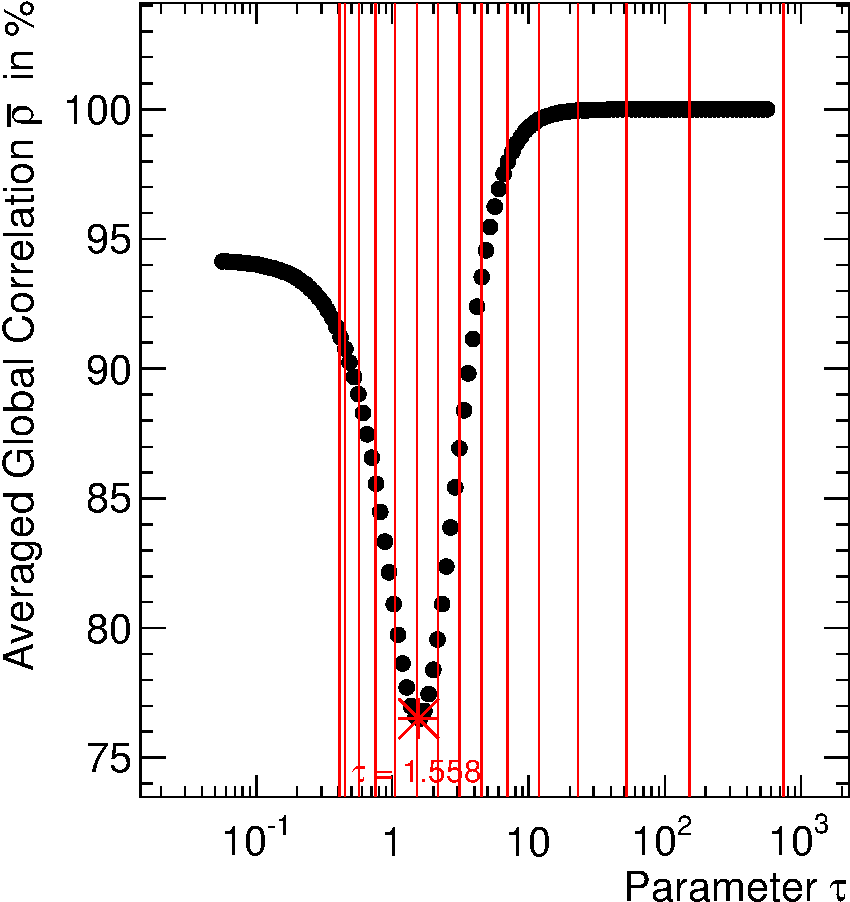
\includegraphics[width=5cm]{ExampleScan}
\par\end{centering}

\centering{}Example Plot for a $\tau$ scan using the averaged global
correlation $\rho$. The mimimum is clearly visible. The vertical
lines indicate the $\tau$ values corresponding to the possible choices
of the discrete $k$-parameter. 
\end{figure}

\par\end{center}


\lyxframeend{}


\lyxframeend{}\lyxframe{Step 7: Unfold With Optimal $\tau$}
\begin{itemize}
\item Now, use the result of the $\tau$ scan for the final unfolding.

\begin{itemize}
\item Turn on file based regularization (1. steering option = 4).
\item Turn off the tau scan (3. steering option = 1).
\item Let the parameter 'regParFile' point to the text file with the optimal
$\tau$ parameters.
\end{itemize}
\end{itemize}

\lyxframeend{}


\lyxframeend{}\lyxframe{Step 8: Customize Your Unfolding}
\begin{itemize}
\item Think about the overflow and underflow bins. Which treatment is best?

\begin{itemize}
\item Check out steering options 10 and 11, see reference guide.
\end{itemize}
\item Do you need to adapt the number of scan points or the scan range?

\begin{itemize}
\item Check out steering options 8 and 9, see reference guide.
\end{itemize}
\item What normalization is right for you?

\begin{itemize}
\item Check out steering option 13, see reference guide.
\end{itemize}
\item Need the results in different formats?

\begin{itemize}
\item Check out steering options 4, 5, 6 and 17, see reference guide.
\end{itemize}
\end{itemize}

\lyxframeend{}


\lyxframeend{}\lyxframe{Step 9: Test the Method}
\begin{itemize}
\item If you unfold your reconstructed MC, do you get back the generated
distribution?

\begin{itemize}
\item Check out steering option 14
\end{itemize}
\item If you reweight your MC to your data and then unfold again, is the
result stable? What happens if you do many such iterations?

\begin{itemize}
\item Check out steering option 15
\end{itemize}
\end{itemize}

\lyxframeend{}


\lyxframeend{}\lyxframe{Step 10: Systematics}
\begin{itemize}
\item If your unfolding runs stable, you can unfold your systematics.
\item If you wish, you can unfold multiple systematics samples at the same
time, by letting the pointer type input parameters be arrays instead
of single histograms. 
\item N\textbf{ote:} \textbf{All pointer type input parameters (except data
input) are expected to be arrays of length 'numSys+1'.} The first
entry will be taken als nominal sample, the following entries as systematics
samples!

\begin{itemize}
\item Example: If you have a nominal, an upshifted and a downshifted sample,

\begin{itemize}
\item set 'numSys' to 2 and let all pointer type parameters be arrays of
length 3 (except data distribution and total data event count).
\item The output parameters 'unfolded' and 'unfoldedNorm' will automatically
arrays of length 3.
\item In addition, the code will produce systematics related control plots.
\end{itemize}
\end{itemize}
\item Note: If you use file based regularization (1. steering option = 4),
all systematic samples will be regularized \textbf{with the same $\tau$
or k parameter} as the nominal sample.
\end{itemize}

\lyxframeend{}


\lyxframeend{}\lyxframe{Your done ...}
\begin{itemize}
\item Congratulations! You did it!
\item Get a cup of coffee and be proud of yourself!
\end{itemize}

\lyxframeend{}
\end{document}
